
%% bare_conf.tex
%% V1.4b
%% 2015/08/26
%% by Michael Shell
%% See:
%% http://www.michaelshell.org/
%% for current contact information.
%%
%% This is a skeleton file demonstrating the use of IEEEtran.cls
%% (requires IEEEtran.cls version 1.8b or later) with an IEEE
%% conference paper.
%%
%% Support sites:
%% http://www.michaelshell.org/tex/ieeetran/
%% http://www.ctan.org/pkg/ieeetran
%% and
%% http://www.ieee.org/

%%*************************************************************************
%% Legal Notice:
%% This code is offered as-is without any warranty either expressed or
%% implied; without even the implied warranty of MERCHANTABILITY or
%% FITNESS FOR A PARTICULAR PURPOSE!
%% User assumes all risk.
%% In no event shall the IEEE or any contributor to this code be liable for
%% any damages or losses, including, but not limited to, incidental,
%% consequential, or any other damages, resulting from the use or misuse
%% of any information contained here.
%%
%% All comments are the opinions of their respective authors and are not
%% necessarily endorsed by the IEEE.
%%
%% This work is distributed under the LaTeX Project Public License (LPPL)
%% ( http://www.latex-project.org/ ) version 1.3, and may be freely used,
%% distributed and modified. A copy of the LPPL, version 1.3, is included
%% in the base LaTeX documentation of all distributions of LaTeX released
%% 2003/12/01 or later.
%% Retain all contribution notices and credits.
%% ** Modified files should be clearly indicated as such, including  **
%% ** renaming them and changing author support contact information. **
%%*************************************************************************


% *** Authors should verify (and, if needed, correct) their LaTeX system  ***
% *** with the testflow diagnostic prior to trusting their LaTeX platform ***
% *** with production work. The IEEE's font choices and paper sizes can   ***
% *** trigger bugs that do not appear when using other class files.       ***                          ***
% The testflow support page is at:
% http://www.michaelshell.org/tex/testflow/



\documentclass[conference]{IEEEtran}

\usepackage[pdftex]{graphicx}
\graphicspath{{../pdf/}{../jpeg/}}
\DeclareGraphicsExtensions{.pdf,.jpeg,.png}
% Some Computer Society conferences also require the compsoc mode option,
% but others use the standard conference format.
%
% If IEEEtran.cls has not been installed into the LaTeX system files,
% manually specify the path to it like:
% \documentclass[conference]{../sty/IEEEtran}





% Some very useful LaTeX packages include:
% (uncomment the ones you want to load)


% *** MISC UTILITY PACKAGES ***
%
%\usepackage{ifpdf}
% Heiko Oberdiek's ifpdf.sty is very useful if you need conditional
% compilation based on whether the output is pdf or dvi.
% usage:
% \ifpdf
%   % pdf code
% \else
%   % dvi code
% \fi
% The latest version of ifpdf.sty can be obtained from:
% http://www.ctan.org/pkg/ifpdf
% Also, note that IEEEtran.cls V1.7 and later provides a builtin
% \ifCLASSINFOpdf conditional that works the same way.
% When switching from latex to pdflatex and vice-versa, the compiler may
% have to be run twice to clear warning/error messages.






% *** CITATION PACKAGES ***
%
%\usepackage{cite}
% cite.sty was written by Donald Arseneau
% V1.6 and later of IEEEtran pre-defines the format of the cite.sty package
% \cite{} output to follow that of the IEEE. Loading the cite package will
% result in citation numbers being automatically sorted and properly
% "compressed/ranged". e.g., [1], [9], [2], [7], [5], [6] without using
% cite.sty will become [1], [2], [5]--[7], [9] using cite.sty. cite.sty's
% \cite will automatically add leading space, if needed. Use cite.sty's
% noadjust option (cite.sty V3.8 and later) if you want to turn this off
% such as if a citation ever needs to be enclosed in parenthesis.
% cite.sty is already installed on most LaTeX systems. Be sure and use
% version 5.0 (2009-03-20) and later if using hyperref.sty.
% The latest version can be obtained at:
% http://www.ctan.org/pkg/cite
% The documentation is contained in the cite.sty file itself.


\usepackage{url}



% *** GRAPHICS RELATED PACKAGES ***
%
\ifCLASSINFOpdf
  % \usepackage[pdftex]{graphicx}
  % declare the path(s) where your graphic files are
  % \graphicspath{{../pdf/}{../jpeg/}}
  % and their extensions so you won't have to specify these with
  % every instance of \includegraphics
  % \DeclareGraphicsExtensions{.pdf,.jpeg,.png}
\else
  % or other class option (dvipsone, dvipdf, if not using dvips). graphicx
  % will default to the driver specified in the system graphics.cfg if no
  % driver is specified.
  % \usepackage[dvips]{graphicx}
  % declare the path(s) where your graphic files are
  % \graphicspath{{../eps/}}
  % and their extensions so you won't have to specify these with
  % every instance of \includegraphics
  % \DeclareGraphicsExtensions{.eps}
\fi
% graphicx was written by David Carlisle and Sebastian Rahtz. It is
% required if you want graphics, photos, etc. graphicx.sty is already
% installed on most LaTeX systems. The latest version and documentation
% can be obtained at:
% http://www.ctan.org/pkg/graphicx
% Another good source of documentation is "Using Imported Graphics in
% LaTeX2e" by Keith Reckdahl which can be found at:
% http://www.ctan.org/pkg/epslatex
%
% latex, and pdflatex in dvi mode, support graphics in encapsulated
% postscript (.eps) format. pdflatex in pdf mode supports graphics
% in .pdf, .jpeg, .png and .mps (metapost) formats. Users should ensure
% that all non-photo figures use a vector format (.eps, .pdf, .mps) and
% not a bitmapped formats (.jpeg, .png). The IEEE frowns on bitmapped formats
% which can result in "jaggedy"/blurry rendering of lines and letters as
% well as large increases in file sizes.
%
% You can find documentation about the pdfTeX application at:
% http://www.tug.org/applications/pdftex

% correct bad hyphenation here
\hyphenation{op-tical net-works semi-conduc-tor}

\begin{document}
\title{Prototyping Resilient Processing Cores in Workcraft}

\vspace{-1mm}
\author{\IEEEauthorblockN{Georgy Lukyanov\IEEEauthorrefmark{2},
Alessandro de Gennaro\IEEEauthorrefmark{3},
Andrey Mokhov\IEEEauthorrefmark{3},
Paulius Stankaitis\IEEEauthorrefmark{3},
Maxim Rykunov\IEEEauthorrefmark{4}}
\IEEEauthorblockA{\IEEEauthorrefmark{2}Southern Federal University, Rostov-on-Don, Russia}
\IEEEauthorblockA{\IEEEauthorrefmark{3}Newcastle University, Newcastle upon Tyne, UK}
\IEEEauthorblockA{\IEEEauthorrefmark{4}IMEC, Leuven, Belgium}
}

\maketitle

% As a general rule, do not put math, special symbols or citations
% in the abstract
\begin{abstract}
We present a methodology for the design and fast prototyping of
processing cores with resilient microarchitecture. The resilience is
achieved by equipping the core with a family of datapath components
optimised for different operating modes and a flexible control
structure that allows to change an instruction implementation in
runtime depending on the environmental conditions and application
requirements. We use asynchronous design techniques to achieve
\emph{short-term resilience}, i.e. survival in extreme environmental
conditions, such as near-threshold and/or unstable voltage supply.
\emph{Long-term resilience} is achieved by providing mechanisms for
runtime reconfiguration of the processor microarchitecture, which
is essential for safety-critical applications, such as biomedical
implants that cannot be taken offline for maintenance. By using
formal methods one can guarantee the correctness and uninterrupted
service during such runtime reconfigurations.

The presented methodology is supported by open-source EDA tool
\textsc{Workcraft}, and has been validated in silicon by successfully
fabricating two chips: Intel 8051 processing core and a
reconfigurable dataflow pipeline for ordinal pattern analysis.
To facilitate fast prototyping of resilient processing cores, we
propose a domain-specific language for formal specification,
compiler-checked documentation, and software-level simulation of
processor prototypes.
\end{abstract}

% no keywords

\IEEEpeerreviewmaketitle
\vspace{-1mm}
\section{Formal methods for resilient systems}
\vspace{-1mm}

Many resilient systems rely on runtime reconfigurability to adapt to
continuously changing environment without any human intervention. For example,
biomedical implants must be able to operate autonomously within patients,
adapting to short-term and long-term changes, with required lifetimes in the
order of decades. Runtime reconfigurability can be achieved both in hardware
and software; the latter is less challenging to implement, however, the former
is often unavoidable. In this paper we focus on hardware reconfigurability.

Formal methods provide a systematic approach for developing complex systems
in a reusable and correct-by-construction manner. The suitability of these
techniques for the specification and verification of reconfigurable
systems has been studied for some time now. We refer the reader to a survey by
Calinescu and Kikuchi~\cite{calinescu2010formal} that overviews the use of
formal methods for adaptive systems at runtime, and an empirical comparison
of different modelling formalisms by
Bhattacharyya et al.~\cite{DBLP:journals/corr/BhattacharyyaMP16}. In the our
work~\cite{ISA-formal} we introduced a methodology for the formal specification
and synthesis of processor microarchitecture with runtime reconfigurability.
The methodology is supported by open-source EDA toolsuite
\textsc{Workcraft}~\cite{workcraft_web} and validated in silicon~\cite{rec-proc}.
In the rest of the paper we discuss our current work on
providing fast prototyping of reconfigurable resilient processing cores in
\textsc{Workcraft} using a domain-specific language for
microarchitecture description (Section~\ref{sec:dsl}), and report on our
experience in designing resilient processing cores using this methodology
(Section~\ref{sec:tools}).

% The authors of the paper~\cite{Weyns:2012:SFM:2347583.2347592}
% review a decade of research on formal
% methods for adaptive systems. Even though the formal verification is traditionally
% an off-line procedure some progress have been achieved in integrating techniques like
% model checking at runtime. The model checking approach involves specifying system behaviour
% formally or else using a model finding approach \cite{kikuchi2010configuration}
% and exhaustively checking that systems properties hold at every system change.
% The counter-examples can be used to resolve the policy conflicts as discussed by
% Calinescu and Kikuchi in their paper. The other methods include using a mathematical logic and theorem prover
% to verify dynamic reconfiguration of cores at a runtime \cite{singh1999formal}. The proposed schema
% automatically generates the new specification of the system in a propositional logic and calls
% the theorem prover at the runtime to check the correctness.

% A lot of safety critical systems
% system has to preserve requirements for resources in case of system failures and in many instances this requires
% reasoning in discrete-continuous domain which is best captured with hybrid models.
% A generic substitution model has been introduced by Babin et al. to reason about reconfigurable
% systems where system state has to be preserved \cite{Babin2016}. The biggest challenge in
% integrating formal verification at runtime is the tool scalability as particularly for
% model checking state-space explosion remains a big challenge.

 %suitable models for analysing
 %discrete-continuous systems are hybrid models. A lot of work has been done to allow
 %modelling such a complex systems and one of the generic models for reconfigurable
 %systems is presented by Babin et al. with a case study for maintaining safe energy
 %level \cite{Babin2016}. The future work direction could involve integrating a similiar
 %approach within our graph-based model.
%Runtime systems adaptation is currently one the biggest challenges in formal
%methods community.
%A number of formal models exists for specification of process-based systems for
%instance Petri nets \cite{peterson1981petri} or Finite State Machines
%\cite{nowick1993automatic} or else hardware description languages such as Verilog or
% VHDL. The majority of industrial projects used formal techniques exactly for the
%specification and modelling as has been shown by Woodcock et al.
%\cite{woodcock2009formal}. The description of application (even formal) is not
%ufficient to evidently demonstrate reliability of the system. The development
%process must be accompanied with a form formal verification and mainly there exists
%two formal verification techniques - theorem proving and model checking. The
%principal of the model checking is to construct a finite-state model and by
%exploring state-space exhaustively check whether the model meets requirements. The
%alternative technique for automated verification is automated theorem proving which
%does not rely on exploring the state-space. The benefits of automated theorem
%proving in hardware design validation are increasingly recognised by the embedded
%system industry \cite{clarke1996formal} and several companies have already
%integrated tools like ACL2 or Isabelle into application development process
%\cite{kaufmann2004some}.

%Our graph-based
%approach combines advantages of PNs and FSMs are is able of capturing concurrency
%and choice in a compact and efficient way.

\section{DSLs for improved design productivity\label{sec:dsl}}

\emph{Domain-Specific Languages} (DSLs) are designed to have a maximal expression for
tasks in a particular domain (for example, VHDL for hardware description or
\LaTeX~for typesetting). However, implementing a language from scratch may be tedious,
time-consuming and error-prone. Therefore, DSLs are often embedded into existing general-purpose programming languages, which is particularly convenient for
prototyping purposes.
Modern functional programming languages such as Haskell offer a
wide range of facilities for construction of \emph{Embedded Domain-Specific Languages}
(EDSLs) that benefit from features of lightweight formal verification provided by
the rich type system and highly-tailored syntax achieved using various functional
programming idioms~[X].

\begin{figure*}[ht!]
\begin{center}
    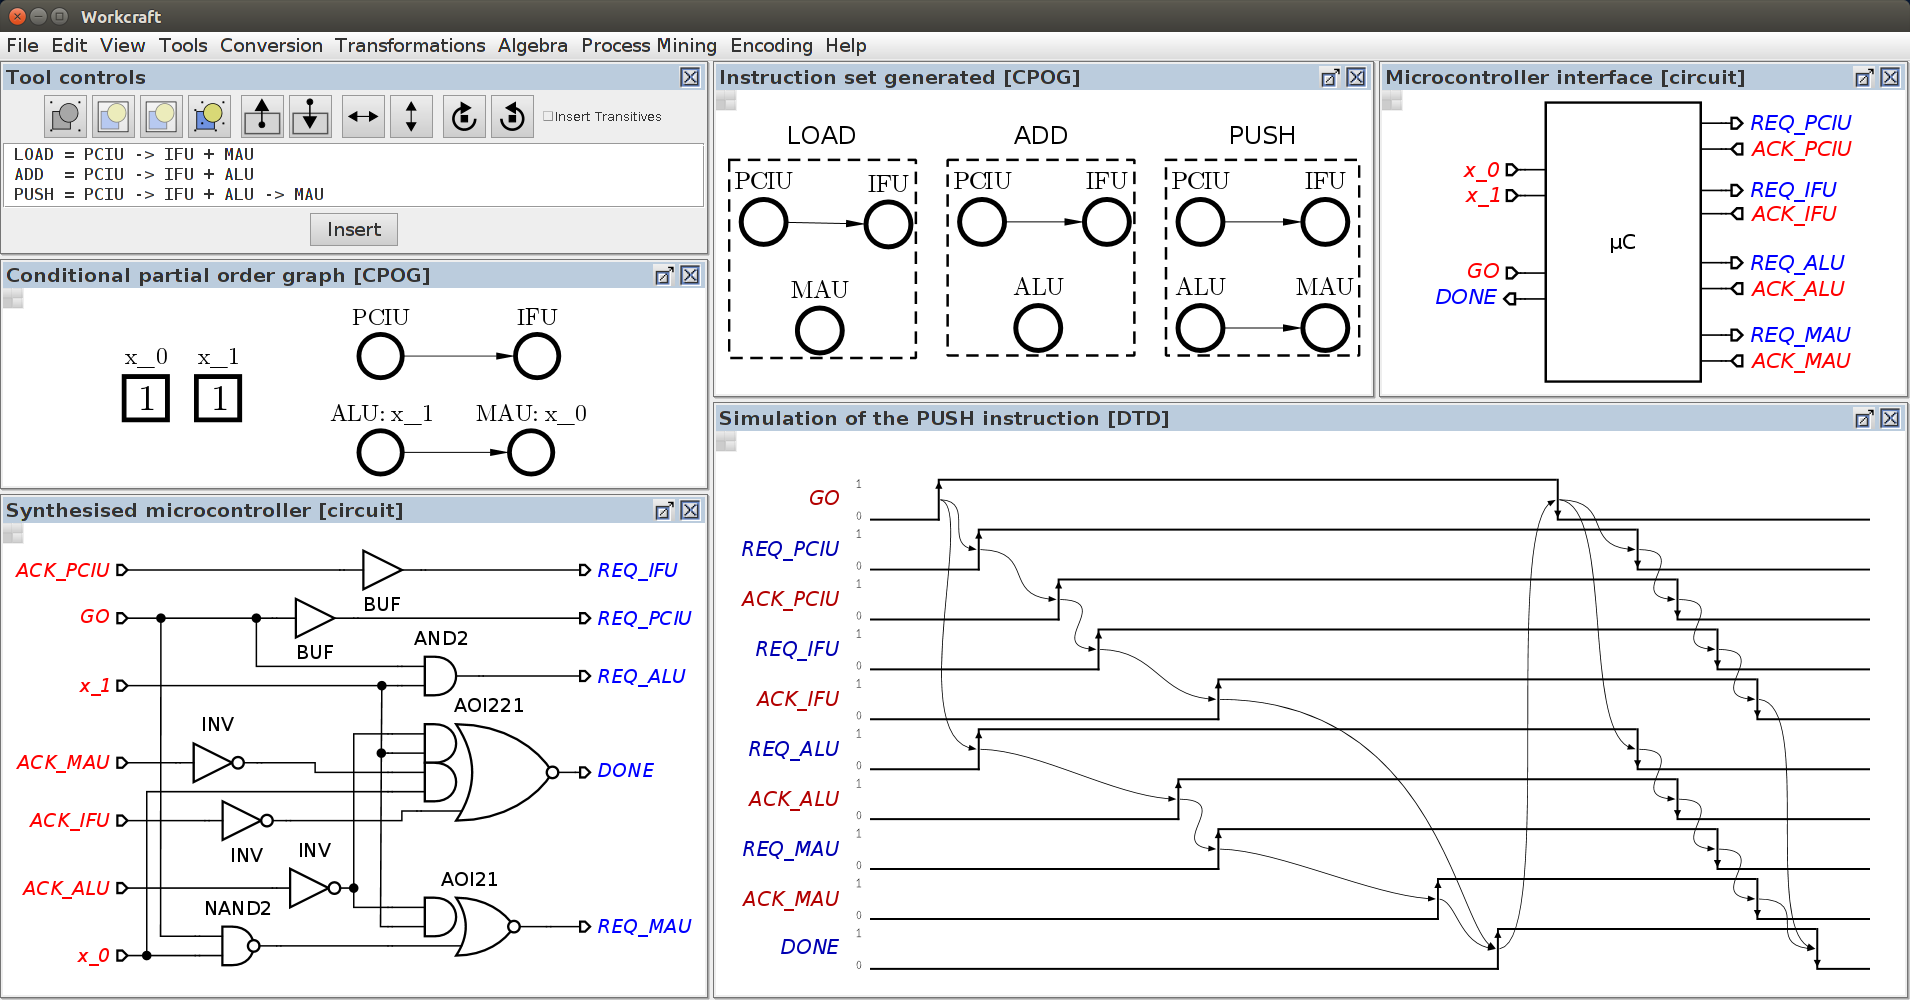
\includegraphics[width=0.95\linewidth]{FIG/screen.png}
    \vspace{-2mm}
    \caption{From the specification of instructions, to the synthesis and simulation
    of the microcontroller. Screenshot from \textsc{Workcraft}.}
    \label{fig:screenshot}
\end{center}
\vspace{-6mm}
\end{figure*}

To design resilient and reconfigurable systems, it is vital to have formal
specification methods, simulation facilities, and verifications techniques.
EDSLs can increase the productivity at every stage of hardware design:
high-level specification
languages help to describe the system functionality in a declarative way, software
simulation environments allow to evaluate the system capabilities
without fabricating an expensive prototype, and advanced types of the host language
provide compiler-checked correctness guarantees for synthesis.

The \textsc{Workcraft} framework provides three DSLs:

\begin{itemize}
\item Signal Transition Graphs (STGs), a signal-level DSL for
specifying resilient asynchronous controllers~\cite{STG}.
\item Conditional Partial Order Graphs (CPOGs), a DSL for specifying
processor microarchitectures~\cite{ISA-formal}.
\item Dataflow Structures (DFSs), a dataflow-level DSL
for specifying dataflow computation graphs~\cite{DFS}.
\end{itemize}

\textsc{Workcraft} can synthesise and export models described in these DSLs into
Verilog, a standard low-level language for hardware description, supported
by conventional tool-chain.

In our work, we focus on bridging Event-B~\cite{EventB}, a high-level DSL
for formal specification of system requirements and reconfiguration,
and DSLs provided by \textsc{Workcraft}. As a prototype of a bridging language,
we develop \emph{Farfalle}, an intermediate-level DSL embedded in Haskell for
the description of reconfigurable processor microarchitectures.
Haskell provides powerful abstractions, e.g. the \texttt{Monad} type class~[Y],
that help to build custom EDSLs with strong static typing and compositional
semantics.

Consider an example illustrating main Farfalle facilities.

\begin{verbatim}
class Monad m => Microprogram m where
    data Register m
    pc, opcode    :: Register m
    readMemory    :: Address -> m Value
    writeMemory   :: Address -> Value -> m ()
    readRegister  :: Register m -> m Value
    writeRegister :: Register m -> Value -> m ()
\end{verbatim}

Here, a microprogram is represented as a typeclass with associated
data type \texttt{Register m}. This class provides abstract interface for
microprogram description. This interface may be
implemented with Haskell's typeclass instances to provide concrete behaviour.
Being a \texttt{Monad}, \texttt{Microprogram m} may be used with
\texttt{do}-notation and able to act as an embedded DSL.

\begin{verbatim}
increment :: Microprogram m => Register m -> m ()
increment register = do
    value <- readRegister register
    writeRegister register (value + 1)
\end{verbatim}

As a result, Farfalle has means to reduce errors in resilient systems design
and give engineers a fast and safe prototyping tool.

\section{Tool support\label{sec:tools}}

Formalising the design specifications is a good approach to the development of a resilient
system. Specifications, represented via DSL, can indeed be verified and
simulated, targeting an error-free system. Workcraft~\cite{workcraft_web} provides the support for different
models, this can help the design for resiliency. Conditional partial order graphs (CPOG)~\cite{ISA-formal}
(available in the Workcraft framework), for instance, can support the development of
processor instruction sets. In Figure \ref{fig:screenshot}, all the steps from the
specification of each instruction, to the synthesis of the final microcontroller are
depicted. Instructions can be specified in the form of algebraic equations at first, then the
graphs can be imported, encoded and synthesised in the form of a microcontroller. The latter
can be mapped with the usage of a technology library and eventually simulated: internal and
external signals can be visualised via digital waveforms, where dependencies among signals
are shown. we are developing a DSL for bridging the gap between formal methods toolsets such
Rodin and hardware synthesis toolsets such as Workcraft. Having a scalable, yet
reusable language would be beneficial for resiliency. The instruction correctness, indeed,
could be simulated and formally verified, the partial order should be derived from the
specifications.

\begin{figure}[h!]
\begin{center}
  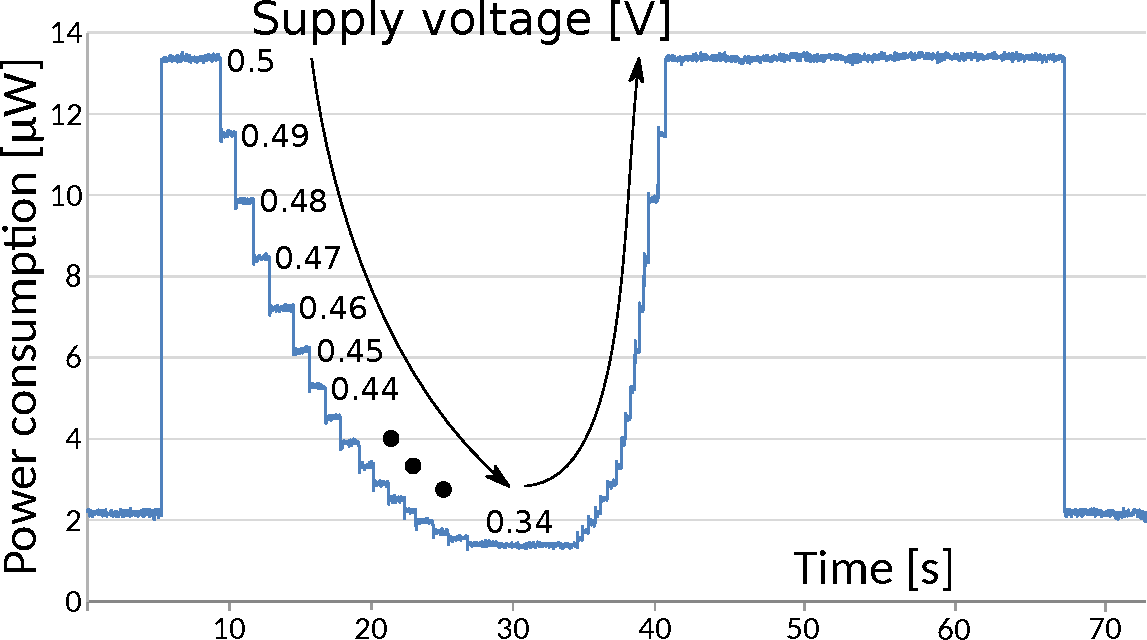
\includegraphics[width=0.8\linewidth]{FIG/ope-chip.pdf}
  \vspace{-3mm}
  \caption{Resiliency of asynchronous control under unstable voltage.}
  \label{fig:voltage-resiliency}
\end{center}
\vspace{-3mm}
\end{figure}


The CPOG and Dataflow Structures (DFS)~\cite{DFS} were used together to design an asynchronous
reconfigurable pipeline for the computation of the ordinal pattern encoding~\cite{OPE}. CPOG was used
for the design of the control unit, which is used for the reconfigurability of the pipeline
(3-18 stages). DFS supported the design of the datapath asynchronous components instead. Each
module has indeed been modelled and simulated in Workcraft at first, and then translated into
hardware description (Verilog). The DFS model matches the HDL description, the asynchronous
4-phase dual rail protocol is implemented. Figure \ref{fig:voltage-resiliency} shows the
resiliency of the chip to the voltage variation. Workcraft, and the tools that the framework
comes with, have been also validated with the design of an asynchronous processor (Intel
8051~\cite{rec-proc}), the flow can still be improved by adopting DSL for formalising system
specifications.

% An example of a floating figure using the graphicx package.
% Note that \label must occur AFTER (or within) \caption.
% For figures, \caption should occur after the \includegraphics.
% Note that IEEEtran v1.7 and later has special internal code that
% is designed to preserve the operation of \label within \caption
% even when the captionsoff option is in effect. However, because
% of issues like this, it may be the safest practice to put all your
% \label just after \caption rather than within \caption{}.
%
% Reminder: the "draftcls" or "draftclsnofoot", not "draft", class
% option should be used if it is desired that the figures are to be
% displayed while in draft mode.
%
%\begin{figure}[!t]
%\centering
%\includegraphics[width=2.5in]{myfigure}
% where an .eps filename suffix will be assumed under latex,
% and a .pdf suffix will be assumed for pdflatex; or what has been declared
% via \DeclareGraphicsExtensions.
%\caption{Simulation results for the network.}
%\label{fig_sim}
%\end{figure}

% Note that the IEEE typically puts floats only at the top, even when this
% results in a large percentage of a column being occupied by floats.


% An example of a double column floating figure using two subfigures.
% (The subfig.sty package must be loaded for this to work.)
% The subfigure \label commands are set within each subfloat command,
% and the \label for the overall figure must come after \caption.
% \hfil is used as a separator to get equal spacing.
% Watch out that the combined width of all the subfigures on a
% line do not exceed the text width or a line break will occur.
%
%\begin{figure*}[!t]
%\centering
%\subfloat[Case I]{\includegraphics[width=2.5in]{box}%
%\label{fig_first_case}}
%\hfil
%\subfloat[Case II]{\includegraphics[width=2.5in]{box}%
%\label{fig_second_case}}
%\caption{Simulation results for the network.}
%\label{fig_sim}
%\end{figure*}
%
% Note that often IEEE papers with subfigures do not employ subfigure
% captions (using the optional argument to \subfloat[]), but instead will
% reference/describe all of them (a), (b), etc., within the main caption.
% Be aware that for subfig.sty to generate the (a), (b), etc., subfigure
% labels, the optional argument to \subfloat must be present. If a
% subcaption is not desired, just leave its contents blank,
% e.g., \subfloat[].


% An example of a floating table. Note that, for IEEE style tables, the
% \caption command should come BEFORE the table and, given that table
% captions serve much like titles, are usually capitalized except for words
% such as a, an, and, as, at, but, by, for, in, nor, of, on, or, the, to
% and up, which are usually not capitalized unless they are the first or
% last word of the caption. Table text will default to \footnotesize as
% the IEEE normally uses this smaller font for tables.
% The \label must come after \caption as always.
%
%\begin{table}[!t]
%% increase table row spacing, adjust to taste
%\renewcommand{\arraystretch}{1.3}
% if using array.sty, it might be a good idea to tweak the value of
% \extrarowheight as needed to properly center the text within the cells
%\caption{An Example of a Table}
%\label{table_example}
%\centering
%% Some packages, such as MDW tools, offer better commands for making tables
%% than the plain LaTeX2e tabular which is used here.
%\begin{tabular}{|c||c|}
%\hline
%One & Two\\
%\hline
%Three & Four\\
%\hline
%\end{tabular}
%\end{table}


% Note that the IEEE does not put floats in the very first column
% - or typically anywhere on the first page for that matter. Also,
% in-text middle ("here") positioning is typically not used, but it
% is allowed and encouraged for Computer Society conferences (but
% not Computer Society journals). Most IEEE journals/conferences use
% top floats exclusively.
% Note that, LaTeX2e, unlike IEEE journals/conferences, places
% footnotes above bottom floats. This can be corrected via the
% \fnbelowfloat command of the stfloats package.


% trigger a \newpage just before the given reference
% number - used to balance the columns on the last page
% adjust value as needed - may need to be readjusted if
% the document is modified later
%\IEEEtriggeratref{8}
% The "triggered" command can be changed if desired:
%\IEEEtriggercmd{\enlargethispage{-5in}}

% references section

% can use a bibliography generated by BibTeX as a .bbl file
% BibTeX documentation can be easily obtained at:
% http://mirror.ctan.org/biblio/bibtex/contrib/doc/
% The IEEEtran BibTeX style support page is at:
% http://www.michaelshell.org/tex/ieeetran/bibtex/
%\bibliographystyle{IEEEtran}
% argument is your BibTeX string definitions and bibliography database(s)
%\bibliography{IEEEabrv,../bib/paper}
%
% <OR> manually copy in the resultant .bbl file
% set second argument of \begin to the number of references
% (used to reserve space for the reference number labels box)

\begin{thebibliography}{10}

\bibitem{calinescu2010formal}
R. Calinescu, S. Kikuchi. \emph{``Formal methods @ runtime''}. In Proceedings of the Monterey Workshop, Pages 122–135, Springer, 2010.

\bibitem{DBLP:journals/corr/BhattacharyyaMP16}
A. Bhattacharyya, A. Mokhov, K. Pierce. \emph{``An Empirical Comparison of Formalisms for Modelling and Analysis of Dynamic Reconfiguration of Dependable Systems''}. Formal Aspects of Computing, Springer, 2016.

\bibitem{ISA-formal}
A. Mokhov et al.
\emph{``Synthesis of processor instruction sets from high-level ISA specifications''}. IEEE Transaction on Computers 2014, vol. 63(6).

\bibitem{workcraft_web}
    \textsc{Workcraft} framework homepage: \url{http://www.workcraft.org/}.

\bibitem{rec-proc}
  A. Mokhov, M. Rykunov, D. Sokolov, A. Yakovlev.
  \emph{``Design of Processors with Reconfigurable Microarchitecture''}.
  J. Low Power Electronics Application, 2014, vol. 4(1), pp. 26-43.

\bibitem{STG}
J. Cortadella et al. \emph{``Logic synthesis for asynchronous controllers and interfaces''}, Springer, 2012.

\bibitem{DFS}
  D. Sokolov, I. Poliakov, A. Yakovlev. \emph{``Analysis of static data flow structures''}. Fundamenta Informaticae, vol. 88(4), pp. 581-610, 2008.

\bibitem{EventB}
  J-R. Abrial. \emph{Modeling in Event-B: system and software engineering}. Cambridge University Press, 2010.

\bibitem{OPE}
  C. Guo, W. Luk, S. Weston:
  \emph{``Pipelined reconfigurable accelerator for ordinal pattern encoding''}.
  IEEE Conference on Application-specific Systems, Architectures and Processors~(ASAP), 2014,
  pp.~194--201.

% \bibitem{Weyns:2012:SFM:2347583.2347592}
% D. Weyns, M. U. Iftikhar, D. G. de la Iglesia, T. Ahmad. \emph{``A
% survey of formal methods in self-adaptive systems''}. In Proceedings of the International C* Conference on
% Computer Science and Software Engineering, C3S2E ’12, (New York, NY, USA), Pages 67–79, ACM, 2012.

% \bibitem{kikuchi2010configuration}
% S. Kikuchi, S. Tsuchiya. \emph{``Configuration procedure synthesis for complex systems using model finder''}.
% In Proceedings of the 15th IEEE International Conference on Engineering of Complex Computer
% Systems (ICECCS), Pages 95–104, IEEE, 2010.

% \bibitem{singh1999formal}
% S. Singh, C. J. Lillieroth. \emph{``Formal verification of reconfigurable core''}.
% Seventh Annual IEEE Symposium on Field-Programmable Custom Computing Machines, 1999. FCCM’99.
% Proceedings. , Pages 25–32, IEEE, 1999.

% \bibitem{Babin2016}
% G. Babin, Y. A{\"i}t-Ameur, N. K. Singh, M. Pantel. \emph{``A System Substi-
% tution Mechanism for Hybrid Systems in Event-B''}.  In Proceedings of the International
% Conference on Formal Engineering Methods, Pages 106-121. Springer International Publishing, 2016.

\end{thebibliography}



% that's all folks
\end{document}
